%!TEX root = ../dissertation.tex

\hypertarget{(chap:capitolo4)}{}
\chapter{Sistemi di raccomandazione}
\section{Introduzione}
Uno dei campi più popolari al momento verso cui si rivolge una particolare attenzione è quello dei sistemi di raccomandazione, da ora in poi RS, in quanto l'attività online sta aumentando sempre più e nascono sempre più spesso nuovi servizi che permettono di scegliere oggetti, siano questi prodotti, video, musica, film o molto altro, da cataloghi vastissimi. I sistemi di raccomandazione permettono di navigare questi cataloghi andando a cercare gli oggetti che risultino più interessanti per l'utente.

\section{Preliminari}
In generale possiamo dire che un RS si compone di diversi elementi, in primo luogo abbiamo i cosidetti "attori" del problema, gli user, ossia gli utenti del sistema, e gli item, ossia gli oggetti che si vuole consigliare. Abbiamo a disposizione inoltre informazioni riguardo l'interazione tra user e item solitamente sotto forma di feedback implicito o esplicito, questa misura viene definito rating. Questi vengono utilizzati dal RS, insieme con eventuali dati legati al contesto di user e item, per effettuare raccomandazioni.

\subsection{Feedback impliciti / espliciti}
Solitamente le informazioni che legano user e item, ossia i rating, possono essere di due tipi:
\begin{itemize}
	\item Implicito: 1 se c'è stata interazione tra lo user e l'item, 0 se non c'è stata;
	\item Esplicito: valutazione numerica intera in una scala da 1 a N, 0 se non c'è stata interazione.
\end{itemize}

Nel nostro caso di studio però ci ritroviamo a metà strada in quanto, la quantità per esempio potrebbe essere considerata come un dato esplicito ma non è definita su una scala discreta, mentre se lo considerassimo implicito trascureremmo delle informazioni che possono in qualche modo fornire una misura di interesse.

\section{User-item interaction matrix}
\begin{minipage}[H]{0.40\textwidth}
	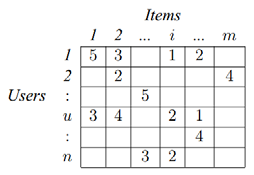
\includegraphics[width=5.5cm]{figures/Sample-of-user-item-matrix}
\end{minipage}
\begin{minipage}[H]{0.55\textwidth}
	I rating sono organizzati in matrici, dette appunto user-item interaction matrix, dove sulle righe abbiamo gli user mentre sulle colonne abbiamo gli item, nell'incrocio abbiamo riportato il rating. 
	Può essere di rating sia impliciti che espliciti e le celle vuote corrispondono allo 0.
\end{minipage}

\section{Task}
L'obiettivo del sistema può essere quello di consigliare ad uno user una lista di N item, detta \textbf{$TopN$} che si ritiene possano interessargli, oppure dato un item si può trovare una lista di item che si considerino simili allo stesso.

\section{Approcci}
Definito quindi il task abbiamo diversi modi per poter soddisfare il nostro obiettivo, in generale abbiamo due principali categorie di RS:
\begin{itemize}
	\item \textbf{Non Personalizzato}: andiamo a consigliare i prodotti che globalmente risultano più popolari, ossia che abbiamo complessivamente ricevuto più valutazioni, o quelli con rating più alto. Questo approccio non va a considerare le informazioni relative il singolo user;
	\item \textbf{Personalizzato}: ci sono diversi approcci che vedremo nelle sezioni successive, in generale si fanno raccomandazioni basate sulle informazioni dello user.
\end{itemize}
I due approcci più famosi negli RS sono il collaborative filtering, dove si cerca di consigliare item ad uno user basandosi su user simili, mentre nel content-based filtering si cerca di raccomandare item simili a quelli con cui si ha già interagito;

\subsection{Collaborative filtering}
Collaborative filtering è un approccio agli RS basato sulla similarità, raccomandiamo ad uno user item interessanti per altri user simili ad esso, e viceversa item simili ad altri item per cui ha dimostrato interesse.
La similarità può essere quindi di due tipi: item-based, basata quindi sulla similarità tra prodotti o user-based ossia su quella tra user.
Ci sono due approcci possibili al collaborative filtering:
\begin{itemize}
	\item Memory-based: utilizziamo la matrice dei rating per calcolare la similarità tra user e item, metodi basati sull'algoritmo K nearest neighbour;
	\item Model-based: utilizziamo dei modelli che attraverso degli algoritmi permettono di predire il rating su item non valutati.
\end{itemize}

\subsubsection{UserKnn}
UserKnn è un metodo memory-based che fa uso della matrice dei rating, ogni user avrà quindi un proprio "profilo", ossia la sua riga nella matrice dei rating. L'idea è quella di calcolare la similarità tra tutti gli user, e per ciascuno di essi selezionare i K più simili.
Una volta fatta questa operazione è possibile calcolare il rating di un prodotto andando 

\subsubsection{ItemKnn}

\subsubsection{Matrix Factorization (MF)}

\subsubsection{Variational Auto-Encoder for CF (VAECF)}

\subsection{Content-based filtering}

